% !TeX spellcheck = cs_CZ
% file: kap_teorie_trafa.tex
{\tikzset{external/prefix={tikz/TEO/}}
 \tikzset{external/figure name/.add={ch08_}{}}
%==================== Kapitola: Teorie transformátoru ==============================================
\chapter{Teorie transformátoru}\label{ES:kap_teorie_trafa}
\minitoc

  Před zahájením studia této kapitoly je naprosto nezbytné nejdříve pročíst kapitolu 
  \ref{teo:IchapII} a seznámit se s \emph{principem reciprocity} v pasivních přenosových 
  soustavách, s \emph{počtem stupňů} volnosti pasivních soustav, s popisem přenosového dvojbranu 
  pomocí matic typu \(\mathbb{Z}\), \(\mathbb{Y}\) a \(\mathbb{H}\) a konečně se základními 
  \emph{přenosovými parametry} dvojbranu.
  
  Zvláštním a neobvyklým cílem této kapitoly je, kromě jiného, podání dvou nezávislých 
  matematických důkazů, že \emph{přesných} náhradních zapojení transformátoru lze sestrojit 
  \emph{nekonečně mnoho}, přičemž pouze dvě z nich, tj. \(\Gamma\)-článek a obrácený 
  \(\ammaG\)-článek mají mimořádný význam. Bude ukázáno, že používání klasického T-článku je sice 
  možné, ale je zbytečně složité! Bude podán matematický důkaz, že lpění na náhradním zapojení v 
  podobě T-článku postrádá jakýkoli fyzikální i matematický smysl a v žádném případě nepřináší 
  žádné výhody \cite[s.~340]{Patocka4}. 

  Problematika transformátoru je rozdělena do dvou základních částí. V první je transformátor  
  představen jako lineární pasivní dvojbran, ve druhé jako nelineární pasivní dvojbran. Postupně  
  bude věnována pozornost následujícím tématům.

  \emph{Transformátor jako lineární pasivní dvojbran}:
    \begin{itemize}\addtolength{\itemsep}{-0.5\baselineskip}
      \item Princip reciprocity. Počet stupňů volnosti.
      \item Názvosloví a klasifikace transformátorů.
      \item Názvosloví a klasifikace přípustných modelů transformátoru.
      \item Základní fyzikální model ve tvaru impedanční \(\mathbb{Z}\)-matice.
      \item Model transformátoru \emph{napětí} ve tvaru hybridní \(\mathbb{H_U}\)-matice.
      \item Model transformátoru \emph{proudu} ve tvaru hybridní \(\mathbb{H_I}\)-matice.
      \item \emph{Ekvivalentní} zapojení transformátoru. Z něho plynoucí experimentální identifikace
            parametrů.
      \item \emph{Náhradní} zapojení transformátoru. Dvě odlišné metody hledání náhradního zapojení:
            \begin{itemize}
              \item metoda separace rozptylových indukčností,
              \item metoda stejné vstupní impedance.
            \end{itemize} 
            Obě metody vedou k témuž výsledku: přesných náhradních zapojení existuje nekonečně 
            mnoho. Lze je rozdělit do dvou tříd: třída fyzikálně \emph{realizovatelných} třída 
            \emph{nerealizovatelných} zapojení (ale přesto matematicky korektních). Vypovídací 
            schopnost náhradního zapojení.
      \item Vztah mezi Hopkinsonovými činiteli rozptylu \(\nu\) a činitelem vazby \(k\).
    \end{itemize}
    
  \emph{Transformátor jako nelineární pasivní dvojbran}:
    \begin{itemize}
      \item Matematický model transformátoru napětí a proudu s nelineární magnetizační  
            charakteristikou feromagnetika, bez uvažování hystereze.
      \item Teoretické zdůvodnění známého experimentálního faktu, že nelinearita magnetizační
            charakteristiky nemá negativní vliv na linearitu \emph{napěťového přenosu} transformátoru.
    \end{itemize}

  %------------ Transformátor jako lineární pasivní dvojbran ---------------------------------------
  \section{Transformátor jako lineární pasivní dvojbran}
    Při řešení drtivé většiny problémů vyskytujících se v technické praxi je možno pohlížet na
    transformátor jako na lineární přenosový dvojbran.  
    \subsection{Předpoklady analýzy}
      Transformátor podle obr. \ref{ES:fig_005} je typickým představitelem  pasivního 
      přenosového dvojbranu. Analýza transformátoru bude provedena za následujících předpokladů:
      \begin{itemize}\addtolength{\itemsep}{-0.5\baselineskip}
        \item Magnetizační charakteristika feromagnetického obvodu je lineární.
        \item Na obrázku je úmyslná odchylka oproti obvyklému značení směru sekundárního proudu.  
              Jeho směr je totiž volen ve shodě s předpokladem, že transformátor je na výstupu 
              zatížen pasivní zátěží pracující ve spotřebičovém režimu, tj. odporem. Jsou-li 
              začátky obou vinutí označeny tečkami, pak pro okamžité hodnoty proudů i napětí jsou 
              orientace všech čtyř šipek správné, tj. ve shodě se skutečností. Toto je důležitý 
              předpoklad, který z psychologického hlediska zvláště studentům velmi usnadňuje 
              analýzu a pochopení činnosti (není pedagogicky vhodné komplikovat analýzu 
              neprůhledným režimem, s aktivní zátěží na sekundáru).
        \item Neexistují vířivé ztráty ve feromagnetiku. Vířivé ztráty však bude možno na základě
              získaných výsledků velmi přesně analyzovat a přidat do modelu transformátoru.
        \item Neexistují hysterezní ztráty ve feromagnetiku. Navíc problém hystereze nepřísluší do
              oblasti lineárních obvodů.
        \item Neexistují Jouleovy ztráty v mědi. Klademe tedy předpoklad \(R_{Cu1} = 0\), \(R_{Cu2}
              = 0\). Tato podmínka však neubírá na obecnosti řešení. Odpor primárního vinutí lze 
              totiž snadno separovat mimo transformátor a myšlenkově zahrnout do vnitřní impedance 
              napájecího zdroje, podobně odpor sekundárního vinutí lze zahrnout do impedance 
              zátěže. Oba odpory je možno do matematického modelu velmi snadno zpětně znovu 
              začlenit.
        \item Nejsou uvažovány parazitní kapacity jednotlivých vinutí ani kapacita mezi oběma vinutími.
      \end{itemize}
      
      \begin{figure}[ht!] %\ref{ES:fig_005}
        \centering
        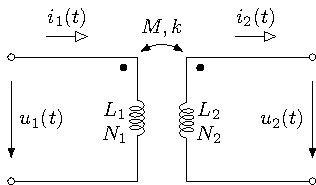
\includegraphics[width=0.5\linewidth]{ES005.pdf}
        \caption{Schématická značka transformátoru. Orientace okamžitých hodnot vstupních a  
                 výstupních signálů s respektováním pasivní zátěže ve spotřebičovém režimu.}
        \label{ES:fig_005}
      \end{figure}

    \subsection{Princip reciprocity u transformátoru}
      Princip reciprocity je nejobecnější vlastností \emph{všech pasivních přenosových soustav}, 
      jak bylo dokázáno v kap. \ref{teo:IchapII}. Princip reciprocity souvisí se známým 
      poznatkem, že \(\mathbb{Z}\)- i \(\mathbb{Y}\)-matice každého lineárního pasivního 
      elektrického obvodu je vždy symetrická podle hlavní diagonály. To znamená, že vždy platí 
      \(z_{ij} = z_{ji}\) a současně \(y_{ij} = y_{ji}\). Všimněme si, že \(\mathbb{Z}\)-matice 
      \ref{ES:eq_MatM02} transformátoru skutečně vyhovuje principu reciprocity, až na znaménko. Obě 
      záporná znaménka v matici jsou důsledkem změny směru proudu \(i_2(t)\) na opačný 
      (realistický), podle obr. \ref{ES:fig_005}, a nejsou na závadu. Platnost principu reciprocity 
      u transformátoru je velmi důležitá, protože v platnosti principu spočívá jediná možnost jak 
      dokázat, že vzájemná indukčnost a činitel vazby transformátoru jsou pro oba směry 
      přenosu stejné, tj. že platí
      \begin{subequations}
        \begin{align}
          M_{12} &= M_{21} = M  \label{teo:eq000a}\\
          k_{12} &= k_{21} = k  \label{teo:eq000b}
        \end{align}
      \end{subequations}
      Oba vztahy jsou neomylně platné pro \emph{„dva jakkoli libovolně v prostoru tvarované vodiče, 
      a to buď bez přítomnosti feromagnetika nebo i společně s ním".} To jest, oba vztahy jsou 
      platné v lineárním prostředí, které však může být magneticky nehomogenní (tj. permeabilita 
      \(\mu\) nemusí být v prostoru konstantní, může být funkcí prostorových souřadnic).
    
      \begin{note}
        Rovnice (\ref{teo:eq000a}), (\ref{teo:eq000b}) totiž obecně vůbec nevyplývají z Neumannova 
        vzorce
        \begin{equation} \label{teo:eq001}
          M = \mu\oint_{l_1}\oint_{l_2}\dfrac{\dd{\vec{l_1}}\cdot\dd{\vec{l_2}}}{r}\,,
        \end{equation}
        pro výpočet vzájemné indukčnosti, jak bývá někdy mylné uváděno. Neumannův vztah je 
        použitelný pouze ve zvláštním případě, jsou-li obě cívky umístěny v magneticky homogenním 
        prostoru s konstantní permeabilitou \(\mu\). V tom případů je pak opravdu důkazem platnosti 
        rovnice (\ref{teo:eq000a}), (\ref{teo:eq000b}) nezávislost výsledku (\ref{teo:eq001}) na 
        pořadí obou integrálů. Neumannův vzorec však nelze použít, vyskytují-li se v okolí cívek 
        dva materiály s rozdílnou pemeabilitou např. vzduch a feromagnetikum, protože ve vzorci 
        musí figurovat konstantní permeabilita \(\mu\).
      \end{note}    
      
    %------------------ Počet stupňů volnosti transformátoru ---------------------------------------
    \subsection{Počet stupňů volnosti transformátoru}

  %--------------------- Matematické modely lineárního transformátoru ------------------------------
  \section{Matematické modely lineárního transformátoru}
    \subsection{Základní model transformátoru ve tvaru \(\mathbb{Z}\)-matice}  
      Pro okamžité hodnoty lze \(\mathbb{Z}\)-matici psát ve tvaru
      \begin{subequations}           
        \label{ES:eq_MatM01}
        \begin{align}
          u_1(t) &= L_1\frac{di_1(t)}{dt} - u_{i1}(t)  \label{ES:eq_MatM01a}\\
          u_2(t) &= u_{i2}(t) - L_2\frac{di_2(t)}{dt}  \label{ES:eq_MatM01b}
        \end{align}
      \end{subequations}
      neboli
      \begin{subequations}
        \label{ES:eq_MatM02}
        \begin{align}          
          \qquad u_1(t) &= L_1\frac{di_1(t)}{dt} 
                                          - M\frac{di_2(t)}{dt}  \label{ES:eq_MatM02a}      \\
                                u_2(t) &=   M\frac{di_1(t)}{dt} 
                                        - L_2\frac{di_2(t)}{dt}  \label{ES:eq_MatM02b}
        \end{align}
      \end{subequations}

  %------------------- Klasifikace a názvosloví transformátoru -----------------------------------  
  \section{Klasifikace a názvosloví transformátoru}

 %--------------------- Souvislost indukovaného napětí a proudu cívkou ----------------------------
  \section{Souvislost indukovaného napětí a proudu cívkou}
    Bylo již řečeno, že časový průběh spřaženého magnetického toku je úměrný integrálu napětí na 
    cívce, nemusí však již být přímo úměrný proudu cívkou. Indukované napětí je jednoznačně určeno 
    rov. \ref{ES:eq_zakl_elm25}. Spřažený magnetický tok je obecnou funkcí proudu cívkou, přičemž 
    proud je
    funkcí času:
    
    \begin{equation}\label{es:eq_tok_proud}
      \Psi(t) = f[i(t)]
    \end{equation}           

    Dosadíme-li rov. \ref{es:eq_tok_proud} do rov. \ref{ES:eq_zakl_elm25} a použijeme-li větu o 
    derivaci složené funkce\footnote{Je-li $y = f(u), u = \varphi(x)$, potom derivace $y$ podle 
    proměnné $x$ je rovna derivaci $y$ podle proměnné $u$, násobené derivací $u$ podle proměnné 
    $x$}, obdržíme pro napětí na cívce:
    \begin{equation}\label{es_tok_deriv}
      u(t) = \frac{d}{dt} f[i(t)] = \frac{\Psi(i)}{di} \frac{di}{dt} = L_d \cdot \frac{di}{dt}
    \end{equation}

    \begin{figure}[ht!]  %\ref{es:fig_mag_char_trafa_fer}
      \centering
      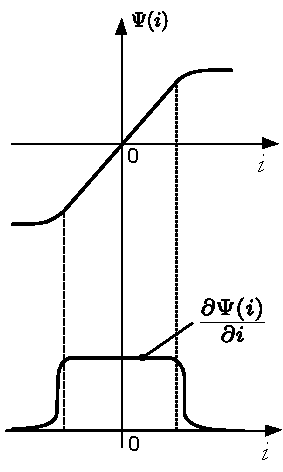
\includegraphics[width=0.4\linewidth]{mag_char_fer.pdf}
      \caption{Statická magnetizační charakteristika transformátoru s feromagnetickým jádrem a 
        závislost diferenciální indukčnosti na proudu. \cite[s.~5]{Elrev2005trafo}}
      \label{es:fig_mag_char_trafa_fer}
    \end{figure}
    
    kde $L_d=\frac{d\Psi(i)}{di}$ má význam \textbf{diferenciální indukčnosti}. Ta může být ve 
    speciálních případech konstantní, ale ve většině reálných aplikací je funkcí proudu cívkou. 
    Jako příklad uvedeme transformátor s feromagnetickým jádrem. Zde je závislost spřaženého 
    magnetického toku na proudu silně nelineárně závislá, obr. \ref{es:fig_mag_char_trafa_fer}. 
    Potom mluvíme o nelineárních magnetických obvodech.

    Na obr. \ref{es:fig_mag_char_trafa_fer} je zobrazena \textbf{statická magnetizační 
    charakteristika} a její derivace, představující průběh diferenciální indukčnosti vinutí v 
    závislosti na proudu. Vidíme, že pro malé proudy je indukčnost největší s rostoucím proudem 
    prudce klesá, nastane-li tzv. přesycení magnetického obvodu transformátoru. Tomuto režimu se 
    snažíme správným návrhem transformátoru vyhnout. Velmi často se v technické praxi zavádí 
    zjednodušení, při kterém se reálný magnetický obvod linearizuje - diferenciální indukčnost je 
    považována za konstantní (nezávislá na proudu cívkou). Mluvíme pak o lineárních magnetických 
    obvodech. Toto zjednodušení je použitelné pouze tehdy, pokud reálný magnetický obvod 
    (transformátor) provozujeme v určitých mezích magnetizačního proudu, kdy se skutečná indukčnost
    příliš nemění. Nelineární magnetizační charakteristika na obr. \ref{es:fig_mag_char_trafa_fer} 
    se linearizuje do podoby na obr. \ref{figure:mag_lin}.

    \begin{figure}[ht!]   %\ref{figure:mag_lin}
      \centering
      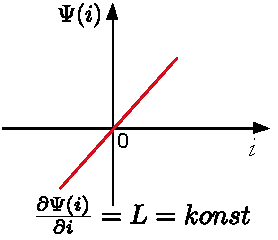
\includegraphics[width=0.5\linewidth]{mag_linearizace.pdf}
      \caption{Linearizovaná magnetizační charakteristika. Směrnice této přímky je právě rovna $L$}
      \label{figure:mag_lin}
    \end{figure}
    Závislost spřaženého magnetického toku na proudu cívkou je tedy lineární ($L=konst$) viz obrázek
    \ref{figure:mag_lin}:
    \begin{equation}\label{es_tok_L}
      \Psi(t)=f[i(t)] = L \cdot i(t)
    \end{equation}    
    Dosazením spřaženého magnetického toku do Faradayova zákona elektromagnetické indukce - rov.
    \ref{ES:eq_zakl_elm25}
    \begin{equation}\label{es_tok_faraday}
        u(t)=\frac{d}{dt}f[i(t)]=\frac{d}{dt}[L\cdot i]=L\cdot\frac{di}{dt}
    \end{equation}
    Ve zvláštním případě stejnosměrných veličin, kdy proud má lineární charakter, přejde vztah
    \ref{es_tok_L} do tvaru, který představuje tzv. \textbf{statickou definici indukčnosti}.
    \begin{equation}\label{es_stat_L}
      \Psi(t)= L \cdot I
    \end{equation}
    Je ale třeba zdůraznit, že rov. \ref{es_tok_L}, rov. \ref{es_tok_faraday} a rov. 
    \ref{es_stat_L} \emph{platí pouze pro lineární magnetické obvody}. Jestliže jsou použity při 
    matematickém popisu transformátorů nebo cívek s feromagnetickým jádrem, je třeba mít na paměti, 
    že tento linearizovaný model lze použít jen v určitém omezeném rozsahu daným skutečnou 
    magnetizační charakteristikou. Nicméně, lineární model transformátoru je pro svou jednoduchost 
    často používán. Čerpáno z článku: \librarianTrafoModel
    
  %--------------- Princip činnosti, základní konstrukční provedení -------------------------------
  \section{Princip činnosti, základní konstrukce}
    \begin{definition}
      \textbf{Transformátor} je elektrický netočivý stroj, který umožňuje pře\-nášet elektrickou 
      energii z jednoho obvodu do jiného pomocí vzá\-jemné elektromagnetické indukce. To znamená, 
      že mění její parametry (napětí, proudy), přitom forma energie na vstupu i výstupu zůstává 
      elektrická.
    \end{definition}

    Transformátory jsou nezbytnou součástí řady elektrotechnických zařízení, počínaje vazebními a 
    napájecími transformátorky sdělovacích a polovodičových zařízení až k transformátorům blokovým 
    a přenosovým, užívaným v energetice. Jejich výkony se pohybují od zlomků VA do stovek MVA. 
    Podobně je tomu s jejich napětími od malých až po vvn. Zásadně transformátory  mohou být jedno 
    nebo vícefázové (obvykle třífázové)

    \begin{figure}[ht!]
      \centering
      \begin{tabular}{c}
      \subfloat[Schématická značka transformátoru s jádrem]{\label{enz:fig_trafo_core_sch}
        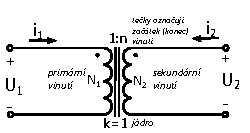
\includegraphics[width=0.7\linewidth]{SCH_Transformer_Core.pdf}}                \\ 
      \subfloat[Principiální provedení transformátoru se dvěma
                vinutími]{\label{es:fig_trafo_core_ideal}
        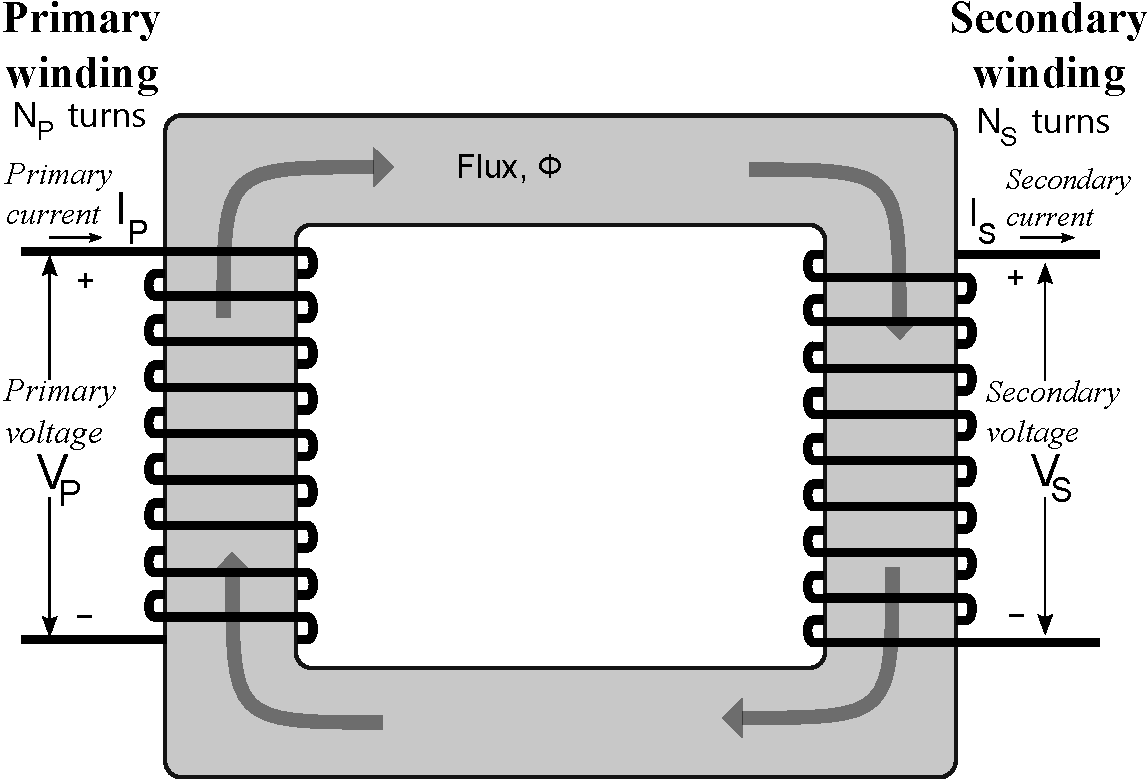
\includegraphics[width=0.8\linewidth]{wiki_single_phase_transformer.pdf}}
      \end{tabular}
      \caption{Ideální transformátor s jádrem, s jedním primárním a jedním sekundárním 
               vinutím. Tečky označují začátky (resp. konce) vinutí. Význam má jejich poloha tečky 
               vůči druhé. Budeme-li je chápat jako začátky vinutí, měl by se drát primáru a 
               sekundáru vinout tak, jak je naznačeno na obrázku}
      \label{es:fig_trafo_ideal}
    \end{figure}
    Princip transformátoru je založen na \textbf{zákonu elektromagnetické indukce} - tedy 
    magnetický tok vybuzený jedním vinutím indukuje napětí ve vinutí druhém (primár, sekundár). 
    Obrázek \ref{es:fig_trafo_core_ideal} ukazuje, že magnetický tok je z jednoho vinutí do druhého 
    veden  prostřednictvím magnetického obvodu. Fyzikální princip vychází z \textbf{2. Maxwellovy
    rovnice} \ref{es:eq_ind_z}.

    Převod transformátoru
    \begin{equation}\label{es:eq_turn_ratio}
        n = \frac{N_1}{N_2}; \quad n=\sqrt{\frac{L_1}{L_2}}
    \end{equation}
    
  %---------------- Zjednodušený rozbor funkce transformátoru -------------------------------------
  \section{Zjednodušený rozbor funkce transformátoru}\label{ES:kap_simple_rozbor_trafa}
    Uvažujme pro začátek transformátor s dokonale těsnou vazbou, tedy s \emph{činitelem vazby
    $k=1$, s nulovým rozptylovým magnetickým tokem a s konečnou velikostí indukčnosti $L_1$ a $L_2$
    primárního a sekundárního vinutí}

    \subsection{Situace při sekundárním vinutí naprázdno}\label{ES:kap_rozbor_trafa}
      Podle indukčního zákona platí pro primární a sekundární napětí
      \begin{subequations}\label{ES:eq_015}
        \begin{align}
          u_1(t)&=\frac{d\Psi_\mu}{dt} 
                 = N_1\frac{d\Phi_\mu}{dt}\label{es_eq_trafo1} \\
          u_2(t)&=\frac{d\Psi_\mu}{dt} 
                 = N_2\frac{d\Phi_\mu}{dt}\label{es_eq_trafo2}  
        \end{align}
      \end{subequations}      
      kde $\Phi_\mu(t)$ je magnetický tok v jádře. Porovnáním rov. \ref{es_eq_trafo1} a rov. 
      \ref{es_eq_trafo2} dostaneme následující rovnici:
      \begin{equation}\label{es_int_uprim_trafo}
          u_2(t)=u_1(t)\frac{N_2}{N_1}
      \end{equation}

      \begin{figure}[ht!]   %\ref{ENZ:fig_003}
        \centering
        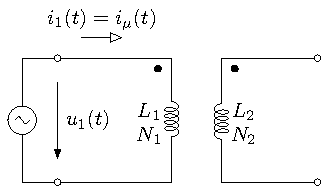
\includegraphics[width=0.5\linewidth]{ES003.pdf}
        \caption{Transformátor naprázdno}
        \label{ENZ:fig_003}
      \end{figure}
      
      Je zřejmé, že $u_1(t)$ a  $u_2(t)$ mohou mít sice různou velikost, ale mají zcela stejný 
      časový průběh. Z rov. \ref{es_eq_trafo1} plyne, že magnetický tok je jednoznačně určen 
      časovým integrálem z přiloženého primárního napětí:
      \begin{equation}\label{es_eq_int_uprim}
          \Phi_\mu(t)=\frac{\int u_1(t)dt}{N_1}+\Phi_{\mu_{poc}}
      \end{equation}
      Primární napětí musí mít nulovou střední hodnotu, tj. nesmí mít stejnosměrnou složku, jinak 
      by magnetický tok rostl nade všechny meze (v praxi do přesycení). Velikost integrační 
      konstanty $\Phi_{\mu_{poc}}$ závisí na konkrétním režimu transformátoru. Z rovnice také plyne 
      užitečný vztah:
      \begin{equation}\label{es_eq_int_uprim_max}
          \Delta\Phi_\mu(t)=\frac{\max|\int u_1(t)dt|}{N_1}
      \end{equation}
      Je-li $u_1(t)$ periodická funkce s nulovou střední hodnotou, pak neurčitý integrál z $u_1(t)$
      je rovněž periodická funkce, jejíž střední hodnota již ovšem nulová být nemusí (viz obr.
      \ref{es:fig_trafo_int_uprim}). $\Phi_\mu$ je rozkmit magnetického toku v jádře transformátoru.
      Z rovnice \ref{es_eq_int_uprim} je patrné, že bez bližší znalosti režimu transformátoru sice 
      nelze přesně stanovit meze, v nichž se magnetický tok periodicky pohybuje, ale dle rov.       
      \ref{es_eq_int_uprim_max} umíme přesně stanovit rozkmit toku čili vzdálenost mezí. Pro 
      předpokládané homogenní rozložení pole ve feromagnetickém jádře lze určit rozkmit magnetické 
      indukce:
      \begin{equation}\label{es_eq_rozkmit_B}
        \Delta B_\mu(t)=\frac{\Delta\Phi_\mu(t)}{S}=\frac{\max|\int u_1(t)dt|}{N_1S}
      \end{equation}

      \begin{figure}[ht!]
        \centering
        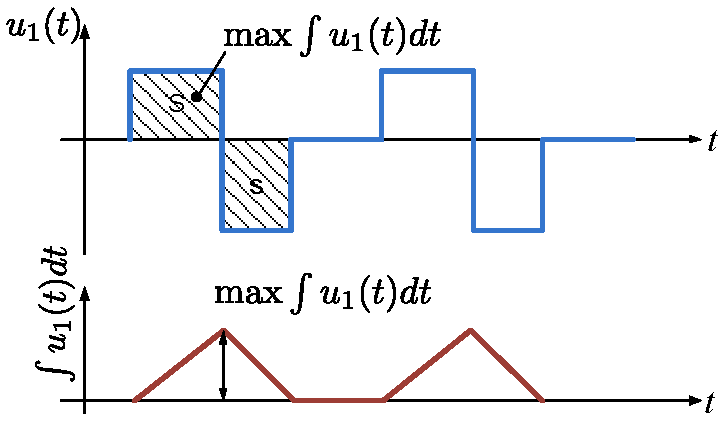
\includegraphics[scale=0.6]{trafo_int_uprim.pdf}
        \caption{Znázornění časového integrálu primárního napětí transformátoru.}
        \label{es:fig_trafo_int_uprim}
      \end{figure}

      pro \emph{lineární} magnetické obvody vztah mezi tokem a magnetizačním proudem:
      \begin{equation}\label{es_eq_stat_def_L}
        N_1\Phi_\mu(t)=L_1i_\mu(t)
      \end{equation}
      Proud $i_\mu(t)$ je primární proud při sekundárním vinutí naprázdno, tzv. 
      \textbf{magnetizační proud}. Je tedy přímo úměrný magnetickému toku $\Phi_\mu(t)$.
      \begin{equation}\label{es_eq_imag}
        i_\mu(t)=\frac{N_1\Phi_\mu(t)}{L_1}
      \end{equation}
      Dosadíme-li za $\Phi_\mu(t)$ rov. \ref{es_eq_int_uprim} uvedené na stránce 
      \pageref{es_eq_int_uprim}, dostaneme známý vztah mezi proudem a napětím cívky, vyjádřený v
      integrálním tvaru:
      \begin{equation}\label{es_eq_imag_u1}
        i_\mu(t)=i_{\mu_{poc}}+\frac{1}{L_1}\int{u_1(t)dt}
      \end{equation}
      Opět vidíme, že primární napětí musí mít nulovou střední hodnotu.
      
    %---------------------------- Situace při zatížení sekundárního vinutí ------------------------
    \subsection{Situace při zatížení sekundárního vinutí}
      Rovnice \ref{es_int_uprim_trafo} až rov. \ref{es_eq_imag_u1} zůstávají v platnosti. 
      Připojíme-li k sekundárnímu vinutí zátěž, začne téci sekundární proud $i_2(t)$. Např. pro 
      odporovou zátěž bude platit
      \begin{equation}\label{es:eq_i2}
        i_2(t)=\frac{u_2(t)}{R_2}
      \end{equation}

      Se sekundárním proudem je svázán magnetický tok $\Phi_2(t)$
      \begin{equation}\label{es:eq_tok_phi2}
        \Phi_2(t)=\frac{L_2i_2(t)}{N_2}
      \end{equation}

      \begin{figure}[ht!]
        \centering
        \begin{tabular}{c}
          \subfloat[Transformátor zatížený]{\label{ES:fig_004a}
            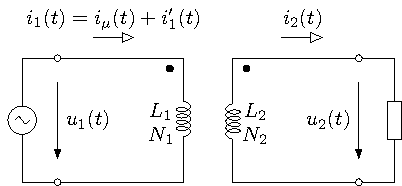
\includegraphics[width=0.9\linewidth]{ES004a.pdf}}             \\
          \subfloat[Zjednodušená představa rozptylu reálného transformátoru]{\label{ES:fig_004b}
            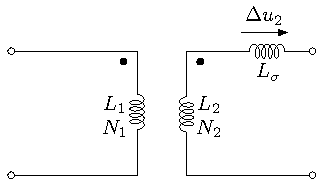
\includegraphics[width=0.7\linewidth]{ES004b.pdf}}             
        \end{tabular}
        \caption{ }
        \label{ES:fig_004}
      \end{figure}
      
      %----------------------------------
      % image: MJ_patocka_trf_Rz.tex label: \label{es:fig_MJ_patocka_trf_Rz}
      %  \input{../src/ES/img/MJ_patocka_trf_Rz.tex}  
      %----------------------------------

      Proud $i_2(t)$, tedy i tok $\Phi_2(t)$, mohou mít bohužel stejnosměrnou složku (zátěží může 
      být např. jednocestný usměrňovač). Stejno\-směr\-nou složku prou\-du však transformátor 
      obecně neumí pře\-trans\-form\-ovat na primární stranu a pak do\-chází ke stejnosměrné 
      před\-magnet\-izaci jádra (sekundární proud stejno\-směr\-nou složku obsahuje, primární proud 
      nikoli). Jedná se o škodlivý jev, který může způsobit, zvláště při větších proudech i 
      přesycení magnetického obvodu. Jev nastává např. při napájení transformátoru ze sítě. Síť se 
      totiž jeví v průběhu celé pracovní periody jako napěťový zdroj s malou vnitřní impedancí. Za 
      zvláštních okolností transformátor stejnosměrnou složku transformovat umí, např. v 
      jednočinném propustném měniči. Zde je transformátor po určitou část periody od primárního 
      zdroje odpojen, v té chvíli se vnitřní impedance primárního zdroje jeví jako nekonečně 
      velká. Oba typy napájení je nutno rozlišovat.

      Dále proto uvažujeme pouze takové typy zátěží, které stejnosměrnou složku ne\-vy\-tvá\-ře\-jí 
      (např. zátěž typu dvoucestný můstkový usměrňovač již tuto nectnost nemá). Pak při uvažování 
      dokonalé vazby, tj. při činiteli vazby $k=1$, je v celém magnetickém obvodu sekundární tok 
      $\Phi_2(t)$ plně vykompenzován primárním tokem $\Phi_1(t)$ stejné velikosti, ale opačného 
      znaménka. Tok $\Phi_1(t)$ je svázán s "přídavným" primárním proudem, tedy proudem 
      pře\-trans\-formovaným ze sekundáru na primár - nazvaný jako $i_1'(t)$. Proud vzniká v 
      primárním vinutí v důsledku Lenzova pravidla. Je zodpovědný za čerpání energie z primárního 
      napájecího zdroje a jeho existence je současně v souladu se zákonem zachování energie

      \begin{equation}\label{es:eq_zachovani_energie}
        \Phi_1(t)=\frac{L_1i_1'}{N_1}=\Phi_2(t)
      \end{equation}

      Srovnáním rov. \ref{es:eq_tok_phi2} a rov. \ref{es:eq_zachovani_energie} obdržíme známý vztah
      pro transformaci proudů:
      \begin{equation}\label{es:eq_i1_cark}
        i_1'(t)=i_2(t)\frac{L_2N_1}{N_2L_1}=i_2 (t)\frac{N_2^2N_1}{N_2N_1^2}=i_2(t)\frac{N_2}{N_1}
      \end{equation}
      Celkový primární proud $i_1(t)$ tedy při zatížení transformátoru sestává ze dvou zcela 
      nezávislých složek. Jednou složkou je magnetizační proud $i_\mu(t)$, který tekl už i ve stavu 
      naprázdno (a nyní při zatížení se nezměnil) a druhou je výše zmiňovaný přetransformovaný 
      proud $i_1'(t)$ :
      \begin{equation}\label{es:eq_i1_sum}
        i_1(t)=i_1'(t)+i_\mu(t)
      \end{equation}
      Z dosud uvedených skutečnosti plyne důležitý závěr: tok v jádře zůstává nezměněn i při 
      zatížení, je tedy stále roven původnímu toku $\Phi_\mu(t)$, protože tok $\Phi_1(t)$ od proudu 
      $i_1'(t)$ a tok $\Phi_2(t)$ od proudu $i_2(t)$ se plně kompenzují. \emph{Sycení jádra u 
      \textbf{bezrozptylového} transformátoru tedy vůbec nezávisí na velikosti zatěžovacího 
      prou\-du, tedy ani na velikosti přenášeného výkonu!}

      Reálné transformátory mají vždy určitý \emph{rozptylový tok}. Ten je svázán s tzv.      
      roz\-pty\-lo\-vý\-mi indukčnostmi (primární a sekundární): Takový transformátor si můžeme 
      představit jako transformátor bezrozptylový s připojen\-ými indukčnostmi $L_{\sigma1}$ do 
      série s pri\-már\-ním vinutím a $L_{\sigma2}$ do série se sekundár\-ním vinutím. Z hlediska 
      vnějšího chování transformátoru lze uvažovat i jedinou rozptylovou indukčnost $L_\sigma$, 
      přepočtenou jen na sekundární stranu (viz obr. \ref{ES:fig_004b}).

      Tento tok je samozřejmě svázán s úbytkem sekundárního napětí $\Delta u_2(t)$ na $L_\sigma$.
      Čili \emph{rozptylová indukčnost způsobuje nenulovou výstupní reaktanci transformátoru},
      Transformátor je pak "\emph{měkký}", zatěžovací proud způsobí úbytek napětí:
      \begin{equation}\label{es:eq_ubytek_Lsigma}
        u_2(t)=N_2\frac{d\Phi_\sigma(t)}{dt}
      \end{equation}
      Skutečný transformátor má navíc nenulové odpory vodičů, na kterých vznikají podle Ohmova
      zákona další úbytky napětí a navíc Joulovy ztráty.

      Vraťme se nyní znovu k transformátoru bezrozptylovému, s dokonalou vazbou, a předpokládejme, 
      že jeho vinutí mají navíc nulový odpor (supravodič). Pak na nich nevzniká průchodem proudu 
      žádný ztrátový výkon a proudy $i_2(t)$  a $i_1'(t)$ lze libovolně zvyšovat. Jejich magnetické 
      účinky se dokonale zruší, nemají tedy vliv na velikost sycení v jádře a transformátorem lze 
      přenášet "libovolně" velký výkon (ve skutečnosti však omezený tzv. kritickou proudovou 
      hustotou supravodiče, při níž zaniká supravodivý jev - pro niob asi 50 A/mm2).

      U měděného (hliníkového) vinutí je nutno volit průřez vodičů úměrný proudu, aby nebyla 
      překročena  dovolená proudová hustota s ohledem na přehřátí vodičů vlivem Joulova tepla. 
      Rovnice \ref{es_eq_rozkmit_B} navíc napovídá, že musíme volit určitý počet primárních závitů 
      $N_1$, abychom nepřekročili maximální sycení jádra. $N_1$ je tím větší, čím je větší maximum 
      - amplituda časového integrálu primárního napětí a čím menší průřez má jádro. Má-li se pak 
      vinutí vtěsnat do okénka jádra, nelze zvyšovat průřez vodiče a tím i proudovou zatížitelnost 
      libovolně. Díky tomu lze s daným průřezem magnetického obvodu $S$ a průřezem okénka $S_0$ 
      realizovat transformátor schopný přenést jen určitý omezený výkon.

      Je tedy zřejmé, že maximální výkon bude přímo úměrný ploše okénka $S_0$, protože čím je $S_0$ 
      větší, tím tlustší vodiče můžeme použít a tím větší proudy (výkon) je možno transformovat. 
      Kromě toho je maximální výkon přímo úměrný i průřezu magnetického obvodu $S$, protože čím je 
      $S$ větší, tím méně závitů $N_1$ potřebujeme pro dané sycení, viz rov. \ref{es_eq_rozkmit_B}, 
      a proto mohou být opět tlustší vodiče. Čili lze napsat:
      \begin{equation}\label{es:eq_Pmax}
        P_{max} \approx S\cdot S_0
      \end{equation}

      Zamyslíme-li se nad rov. \ref{es_eq_rozkmit_B}, lze úměru rov. \ref{es:eq_Pmax} ještě 
      doplnit. Maximální hodnota sycení tj. maximum funkce $B(t)$ je přímo úměrná maximu funkce 
      časového integrálu primárního napětí. Uvažujme, že napětí neobsahuje stejnosměrnou složku, je 
      periodické s kmitočtem $f$, ale jinak libovolného tvaru, tj. libovolného obsahu vyšších 
      harmonických.

      Pak je maximum časového integrálu takového primárního napětí (maximum toku, amplituda toku) 
      zcela jistě konečné a nepřímo úměrné kmitočtu. To znamená, že zvýšíme-li kmitočet n-krát při 
      zachování amplitudy a tvaru napětí, klesne maximum integrálu n-krát a bude moci být dle rov. 
      \ref{es_eq_rozkmit_B} také n-krát méně závitů $N_1$, aby sycení zůstalo stejné. Pak ve 
      stejném poměru n můžeme zvýšit průřez vodičů, aniž bychom se báli, že se vinutí nevejde do 
      okénka. Lze pak přenášet n-krát větší proud a výkon (napětí se nezměnila, pouze vzrostl 
      kmitočet). Čili maximální výkon je přímo úměrný kmitočtu. Rovnici \ref{es:eq_Pmax} lze proto 
      doplnit:
      \begin{equation}\label{es:eq_Pmax2}
        P_{max} \approx f\cdot S\cdot S_0
      \end{equation}
      Pro jádra z plechu EI z křemíkové oceli lze pomocí tohoto vztahu s uvažováním přímé úměry 
      mezi $S_0$ a $S$, odvodit vztah
      \begin{equation}\label{es:eq_Pmax_EI}
        P_{max} \approx S^2\quad [W, cm^2]
      \end{equation}
      Ten předpokládá maximální sycení $1 T$, proudovou hustotu asi $2,5 A/mm^2$ a kmitočet $50 
      Hz$. A týká se opravdu jen EI jader, protože při jeho odvození byla uvažována konkrétní 
      závislost mezi $S_0$ a $S$ pro tato jádra.

      Ze vztahu rov. \ref{es:eq_Pmax2} vidíme, že zvyšování pracovního kmitočtu umožňuje přenášet 
      větší výkon při zachování rozměrů jádra. To je základem filosofie všech spínaných zdrojů 
      (měničů) s transformátorem. Kmitočet však nelze u reálného transformátoru zvyšovat nade 
      všechny meze. Omezení představují hysterezní a vířivé ztráty v jádře a dále rozptylová 
      indukčnost.

  \section{Ztráty v reálném transformátoru}
    \subsection{Joulovy ztráty ve vinutí}
      Joulovy (ohmické) ztráty vznikají na odporu vinutí průchodem proudu. Tato sku\-te\-čnost nutí 
      zvyšovat průřez vodičů a způsobuje tak nutné zvyšování plochy okénka jádra $S_0$ a zvětšování 
      celého transformátoru.

      Z hlediska těchto ztrát se primární a sekundární vinutí chovají jako lineární odpory $R_1$ a 
      $R_2$. Joulovy ztráty jsou proto úměrné kvadrátu efektivní hodnoty procházejícího proudu a 
      jsou dány vztahem:
      \begin{equation}\label{es_joul_loss}
        P_R= R_1 I_{1_ef}^2 + R_2 I_{2_ef}^2
      \end{equation}

      Efektivní hodnota proudů procházejících vinutími obecně není úměrná přenášenému činnému 
      výkonu a může být v praxi někdy nečekaně vysoká. Např. u síťového transformátoru se 
      sekundárním usměrňovačem a filtračním kondenzátorem bez vyrovnávací nárazové tlumivky. Zde 
      odebíraný sekundární proud $i_2(t)$ a tedy přetransformovaná složka primárního proudu 
      $i_1'(t)$ tvar úzkých nabíjecích impulsů s velkou amplitudou. Jeho celková efektivní hodnota 
      je několikrát větší než efektivního hodnota užitečné 1. harmonické, která se v tomto případě 
      pouze samotná podílí na přenosu činného výkonu. Ten je totiž dán součinem efektivní hodnoty 
      harmonického sekundárního napětí, efektivní hodnoty pouze 1. harmonické sekundárního proudu a 
      $\cos\phi$ oné 1. harmonické proudu!

      Pro omezení ohřevu vinutí na přípustnou mez je nutno omezit odpory vinutí. Při návrhu 
      pracujeme s tzv. dovolenou proudovou hustotou $J$. Teče-li proud rovno\-měr\-ně celou plochou 
      průřezu vodiče, platí vztahy:
      \begin{equation}\label{es_proud_hustota}
        J_1=\frac{I_{1_{ef}}}{S_1} \quad J_2=\frac{I_{2_{ef}}}{S_2}
      \end{equation}
      $S_1$ a $S_2$ jsou průřezy primárního  a sekundárního vinutí.

      Doporučená hodnota $J$ se pohybuje v případě měděných vodičů v rozmezí $1,5$ až $7 A/mm^2$. 
      Pro větší transformátory s velkým objemem vinutí je třeba volit vždy hustotu menší. Při 
      \emph{konstantní proudové hustotě totiž celkový Joulův ztrátový výkon roste s třetí mocninou 
      lineárních rozměrů cívky, chladící povrch pouze s druhou mocninou}. Vinutí těsně pod 
      chladícím povrchem mohou mít větší proudovou hustotu než vinutí vnitřní.

      Bez nuceného proudění vzduchu volíme u toroidních transformátorů hustotu $J$ v rozsahu $2$ až
      $5 A/mm^2$, podle velikosti a počtu vrstev vinutí. U malých hrníčkových feritových jader lze 
      volit nouzově až $4,5 A/mm^2$. U běžně užívaných síťových transformátorů s mnohovrstvými 
      cívkami vinutými na kostrách se doporučuje hodnota $1,5 A/mm^2$ (pro velké transformátory) až 
      $3,5 A/mm^2$ (pro malé transformátorky). Při použití nuceného proudění vzduchu může být 
      hustota $J$ větší.

      U transformátorů pracujících na vysokém kmitočtu musíme počítat s uplatněním 
      \textbf{skinefektu}, díky němuž proud teče jen ve vrstvě pod povrchem vodiče a střední část 
      tlustého vodiče by tak byla nevyužita.

    \subsection{Hysterezní ztráty v jádře} %\label{ES:ssec_02}\hypertarget{ENZ:ssec_02}
      Hysterezní ztráty souvisejí s energií $W$ potřebnou na přemagnetování jádra. Energie $W$ je 
      úměrná ploše hysterezní smyčky (viz. obr. 3.5). Plocha hysterezní smyčky má fyzikální rozměr 
      $J/m^3$, jedná se tedy o objemovou hustotu ztrátové energie. Ta je pak  velká pro materiály 
      magneticky tvrdé, se širokou hysterezní smyčkou tj. s velkou \emph{remanencí} $B_R$ a 
      \emph{koercitivní intenzitou} $H_C$. Takové materiály proto nejsou pro jádra transformátoru 
      vhodná. Naopak požadujeme materiály magneticky měkké, s co nejužší hysterezní smyčkou a s co 
      nejmenší remanentní indukcí.

      Je zřejmé, že velikost plochy hysterezní smyčky $S$ a tedy i energie $W$ souvisí nejen s 
      vlastnostmi materiálu $B_R$ a $H_C$, ale i s amplitudou indukce $B_m$. Přibližně platí, že 
      plocha $S$ je úměrná kvadrátu $B_m$.(viz. obr. 3.5). Hysterezní ztrátový výkon je dán 
      součinem této energie $W$ a pracovního kmitočtu $f$, v jehož „rytmu“ dochází k 
      přemagnetovávání.

      \begin{equation}\label{ES:eq_hyster_loss}
        P_h = W \cdot f \approx B_m^2 \cdot f^2
      \end{equation}

      \begin{figure}[ht!]
        \centering
        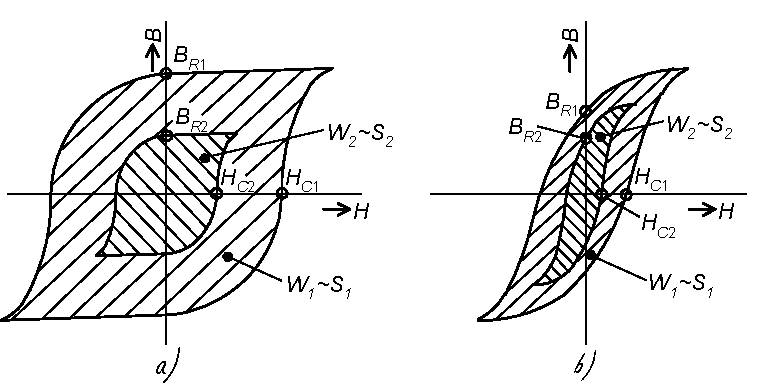
\includegraphics[width=1\linewidth]{patocka_BH_curve.pdf}
        \caption[Hysterezní smyčka feromagnetického materiálu]{Hysterezní smyčka feromagnetického
                 materiálu: a) magneticky tvrdý materiál, b) magneticky měkký materiál.}
        \label{es:fig_BH_curve}
      \end{figure}

      \begin{itemize}
        \item Budeme-li měnit kmitočet a současně zachovávat sycení, tzn. budeme udržovat  
              konstantní poměr amplitudy  $u_1(t)$ a kmitočtu $f$ při proměnném počtu závitů $N_1$ 
              – viz rozbor vztahu (\ref{es_eq_rozkmit_B}). Pak bude díky konstantnímu sycení $B_m$ 
              i konstantní energie $W$. Ze vztahu (\ref{ES:eq_hyster_loss}) je pak vidět, že 
              hysterezní ztráty budou přímo úměrné kmitočtu.
              \begin{equation}\label{ES:eq_hyst_loss_linf}
                P_h \approx f
              \end{equation}
              Toto je typický případ transformátoru v pulsních měničích, kdy volíme vysoký kmitočet 
              za účelem snížení  $N_1$ (aby se vinutí mohlo vinout tlustším vodičem) při zachování 
              (nepřekročení) dovoleného sycení.
        \item Měníme-li kmitočet a současně zachovávat týž transformátor (totéž $N_1$ a $S$) a  
              tutéž amplitudu $u_1(t)$. Pak z rozboru vztahu (\ref{es_eq_rozkmit_B}) vyplývá, že 
              indukce bude nepřímo úměrná kmitočtu.  Čili ze vztahu (\ref{ES:eq_hyster_loss}) pak 
              vidíme, že hysterezní ztráty budou \emph{hyperbolicky}, nepřímo úměrně, klesat s 
              rostoucím kmitočtem.
              \begin{equation}\label{ES:eq_hyst_loss_hypf}
                P_h \approx \frac{1}{f}
              \end{equation}
              Tento režim transformátoru se nazývá \emph{odbuzovací}, neboť při růstu kmitočtu 
              klesá indukce. V pulsních měničích by ale takový režim neměl žádný význam, protože 
              bychom sice zvýšili kmitočet, ale museli bychom použít stále stejný objemný a těžký 
              transformátor s velkým $N_1$, stanoveným pro původní nízký kmitočet.
      \end{itemize}

    \subsection{Ztráty vířivými proudy v jádře}\label{ES:ssec_03}\hypertarget{ES:ssec_03}
      Tyto ztráty jsou způsobeny indukováním napětí v jádře transformátoru. Je-li totiž jádro 
      elektricky vodivé, lze si ho představit jako soustavu nekonečně mnoha soustředných tenkých 
      diferenciálních smyček (jeden závit), vykazujících diferenciální elektrické odpory a 
      protékaných příslušným příspěvkem magnetického toku v jádře transformátoru. Situaci lze 
      přibližně namodelovat představou jediného závitu s elektrickým odporem \(R_v\), obepínajícího 
      celý průřez jádra, tj. celý tok \(\Phi_\mu\). V tomto závitu se pak indukuje napětí 
      (neuvažujme znaménko):
      \begin{align}
        u_i(t) &= \der{\Phi_\mu(t)}{t}  \label{ES:eq_014} \\
        \shortintertext{Srovnáním se vztahem (\ref{es_eq_trafo1}) pak vidíme, že platí:}
        u_i(t) &= \frac{u_1(t)}{N_1}   \label{ES:eq_016} \\
        \shortintertext{A protože odpor \(R_v\) je z principu lineární (železo je elektricky 
                        lineární), budou vířivé ztráty dány vztahem:}
        P_v    &= \frac{U_{ief}^2}{R_v}    \label{ES:eq_017}
      \end{align}
      Aby byly co nejmenší, musí být odpor \(R_v\) co největší, tj. co největší měrný odpor 
      materiálu jádra.
      \begin{itemize}
        \item budeme nyní opět měnit kmitočet za podmínky zachování sycení (tj. současná změna 
              \(N_1\) nebo amplitudy napětí). Ze vztahu (\ref{ES:eq_016}) je pak jasné, že 
              amplituda \(ui(t)\) bude přímo úměrná kmitočtu. Pak vířivé ztráty (\ref{ES:eq_017}) 
              musí být úměrné kvadrátu kmitočtu.
              \begin{equation}\label{ES:eq_018}
                P_v \approx f^2
              \end{equation}
        \item Při odbuzovacím režimu, kdy zvyšujeme kmitočet při zachování transformátoru (\(N_1\)) 
              a amplitudy napětí \(u_1(t)\), \(u_i(t)\) se podle (\ref{ES:eq_014}) vůbec nemění. 
              Čili ztráty vířivými proudy jsou zde konstantní, kmitočtově nezávislé. Opět 
              zdůrazněme, že tento režim nemá v měničích smysl.
      \end{itemize}
      
    \subsection{Volba materiálu jádra}\label{ES:ssec_04}
      V kapitole \ref{ES:ssec_02} jsme ukázali, že materiál jádra musí být magneticky měkký. V kap. 
      \ref{ES:ssec_03} jsme pak zjistili, že měrný odpor materiálu jádra musí být co největší.
      Dalším požadavkem na jádro je co největší dovolené sycení (čili hysterezní smyčka sice úzká, 
      ale vysoká), aby bylo možno volit co nejmenší počet závitů.
    
  \section{Rozptyl transformátoru}
    Vraťme se nyní k zjednodušenému modelu rozptylu z obr. \ref{ES:fig_004b}. Pro velikost
    roz\-ptyl\-ové indukčnosti $L_\sigma$ platí:
    \begin{equation}\label{es:eq_Lsigma}
      L_\sigma=\lambda_\sigma\cdot N_2^2
    \end{equation}
    kde $\lambda_\sigma$ je \emph{magnetická vodivost rozptylového magnetického obvodu}. 
    Rozptylovou indukčnost $L_\sigma$ (tj. sekundární rozptylovou indukčnost plus primární 
    rozptylovou indukčnost přepočtenou na sekundární stranu) je nutno chápat jako indukčnost 
    určující výstupní reaktanci transformátoru napájeného ovšem z ideálního napěťového primárního 
    zdroje. Lze ji snadno změřit, zkratujeme-li primární vinutí a měříme sekundární indukčnost
    $L_{2,k}$:
    \begin{equation}\label{es:eq_L2k}
      L_\sigma=L_{2,k}= L_2(1-k^2)
    \end{equation}
    kde $k$ má význam \emph{činitele vazby} a lze jej určit ze známého vztahu:
    \begin{equation}\label{es:eq_cinitel_vazby}
      k=\frac{M}{L_1L_2}
    \end{equation}
    Zajímá nás ovšem \textbf{výstupní reaktance} $\omega L_\sigma$, nikoliv samotná indukčnost 
    $L_\sigma$, neboť napěťový úbytek je úměrný (při harmonickém průběhu napětí):
    \begin{equation}\label{es:eq_nap_ubytek}
      \Delta u_2(t)\approx \omega L_\sigma
    \end{equation}
    Je zřejmé, že při konstantní rozptylové indukčnosti může být transformátor na vysokých 
    kmitočtech naprosto nepoužitelný (měkký). Pak nezbývá, než velmi ú\-zkost\-li\-vě a co nejvíce 
    minimalizovat rozptylovou indukčnost. Je proto nutné podle rov. \ref{es:eq_Lsigma} 
    minimalizovat rozptylovou magnetickou vodivost $\lambda_\sigma$. Ta je přibližně určená rovnicí:
    \begin{equation}\label{es:eq_rozptyl_vodivost}
      \lambda_\sigma= \mu_0\frac{S_\sigma}{l_\sigma}
    \end{equation}
    kde $\mu_0=4\cdot\pi10^{-7}H/m$ je \emph{permeabilita vakua}. $S_\sigma$ a $l_\sigma$ jsou
    \textbf{ekvivalentní průřez} a \textbf{délka rozptylových cest}. Protože nelze snížit  
    permeabilitu vzduchu, je nutno upravit geometrii jádra a současně zabezpečit co největší poměr 
    permeability jádra k permeabilitě okolního prostředí. Jádro musí mít tvar bez ostrých zlomů ve 
    směru magnetického toku, nejlépe kruhový tvar, tj. \emph{toroidní jádro}. Je důležitá velká 
    magnetická vodivost jádra $\lambda$. Ta je dána vztahem:
    \begin{equation}\label{es:eq_vodivost_jadra}
      \lambda= \mu_r\mu_0\frac{S}{l}
    \end{equation}
    $\mu_r$ je \emph{relativní permeabilita materiálu}, $S$ je \emph{průřez jádra}, $l$ je 
    \emph{délka střední siločáry}. Nestačí jen velká permeabilita  $\mu_r$, ale i velký poměr 
    $\frac{S}{l}$. Pro minimalizaci rozptylu jsou proto vhodná "baculatější" jádra s velkým $S$ a 
    malým $l$ (často například několik toroidů s malým průměrem tj. malým $l$ paralelně pro 
    dosažení velkého $S$). Tím ale vzniká problém malého okénka $S_0$ pro vinutí, což znemožňuje 
    vinout vodiči s velkým průřezem a přenášet tak velké výkony. Tyto protichůdné požadavky na tvar 
    jádra bývají kritické a je nutno je v návrhu kompromisně vyřešit.

    Rozptylovou indukčnost dále zmenšíme způsobem vinutí. Jsou-li vinutí na kostřičce, pak je 
    vineme na sebe, nikoliv vedle sebe s přepážkou. Blíže jádru umístíme vinutí s menším počtem 
    závitů. Vhodné je také střídavé prokládání jednotlivých vrstev primárního a sekundárního 
    vinutí, roste však neúměrně pracnost (cena) a klesá činitel plnění okénka. \emph{Bifilární 
    vinutí} s nejtěsnější vazbou nelze uskutečnit v případě rozdílných počtů závitů (což je téměř 
    vždy) a v případě nároků na izolační pevnost mezi vinutími rozprostřenými rovnoměrně po obvodu 
    celého toroidu.

    \begin{note}
      \textbf{Poznámka k transformátorům obecně (nejen síťovým)}:
      \newline Všimněme si, že v celém výkladu není nikde zmínka o použití \texttt{vzduchové mezery 
      v 
      magnetickém obvodu jádra}. V kapitole Cívky s feromagnetickým jádrem je zamyšlení o 
      vzduchových mezerách v magnetických obvodech a je zde vysvětlen jediný případ, kdy má smysl 
      mezeru v transformátoru použít. Je zde ukázáno, že v případě předpokladu platnosti rov. 
      \ref{es_eq_int_uprim_max} (což je mimo jiné případ běžných napájecích transformátorů) je 
      použití vzduchové mezery bezúčelné a škodlivé, vede totiž ke vzrůstu magnetizačního proudu a 
      zvýšení rozptylových toků.
    \end{note}

  \section{Cívky s feromagnetickým jádrem}
    \subsection{Fyzikální rozbor a příprava pro návrh}\label{ES:ssec_01}
      Cívky s feromagnetickým jádrem se používají k různým účelům. Mohou sloužit jako vyhlazovací
      tlumivky v obvodech ss. proudu, nebo jde o cívky použité v obvodech se střídavým proudem 
      (např. zářivková tlumivka) anebo o nějakou vf. aplikaci v pulsně řízených měničích. Existuje 
      proto celá řada metod návrhu, lišících se podle účelu. Mají samozřejmě stejnou fyzikální 
      podstatu, ale zaměřují se vždy na jiné kritérium, které je pro daný účel podstatné (přesná 
      hodnota indukčnosti, nepřekročení určitého sycení, nezávislost indukčnosti na proudu, malé 
      ztráty, vysoká jakost atd.).
      
      Provedeme návrh cívky s feromagnetickým jádrem vyplývající z jednoduchého fyzikálního rozboru.
      Požadujeme cívku s indukčností \(L\). Známe průběh proudu cívkou \(i(t)\) a jeho maximální 
      (špičkovou) hodnotu \(I_m\). Chceme navrhnout vhodné jádro, počet závitů a vodič vinutí. 
      Maximální indukce v jádře, kdy ještě nedochází k přesycení nechť je \(B_m\).
      
      Pro napětí na cívce určitě platí:
      \begin{align}
        u(t)    &= N\der{\Phi(t)}{t} = L\der{i(t)}{t}            \label{ES:eq_001}  \\
        \shortintertext{\(\Phi(t)\) je magnetický tok v jádře cívky. Integrací (\ref{ES:eq_001}) 
                       dostáváme velmi užitečnou rovnici:} 
        \Psi(t) &= N\Phi(t) = Li(t)                              \label{ES:eq_002}  
      \end{align}
      Přitom \(\Psi(t)\) je tzv. \emph{spřažený magnetický tok v jádře}. Dále platí vztah mezi 
      indukcí a tokem (za \emph{předpokladu homogenního magnetického pole}):
      \begin{equation}\label{ES:eq_003} 
        \Phi(t) = B(t)S
      \end{equation}
      Nechť má cívka zadánu indukčnost \(L\) a maximální proud \(I_m\). Pak z rovnic 
      (\ref{ES:eq_002}) a (\ref{ES:eq_003}) lze získat vztah pro počet závitů, aby nedocházelo k 
      přesycování:
      \begin{equation}\label{ES:eq_004}
        N = \frac{LI_m}{\Phi_m} = \frac{LI_m}{B_mS} 
      \end{equation}
      Vztah říká, jaký počet závitů \(N\) musí mít cívka s indukčností \(L\), aby při maximu proudu 
      \(I_m\) byla v jádře o průřezu \(S\) indukce \(B_m\). Současně platí vztah:
      \begin{equation}\label{ES:eq_005}
        \Lambda = \frac{L}{N^2} 
      \end{equation}
      \(\Lambda\) je magnetická vodivost magnetického obvodu cívky. Anglosaské literatuře se značí 
      \(A_L\). Požadujme tedy velikost této vodivosti podle vztahu (\ref{ES:eq_005}), aby při počtu 
      závitů \(N\) určeném podle (\ref{ES:eq_004}) měla cívka skutečně požadovanou indukčnost \(L\).
      
      Zvolme magnetický obvod cívky tvořený feromagnetickým jádrem se vzduchovou mezerou. Důvody
      této volby vysvětlíme později. Celkový magnetický odpor obvodu nyní bude:
      \begin{align}
        R_m    &= \frac{1}{\Lambda} = R_{Re} + R_v      \label{ES:eq_006} \\ 
        \shortintertext{Přitom \(R_{Fe}\) je magnetický odpor feromagnetické části a \(R_v\) je 
                        magnetický odpor mezery.}
        R_{Fe} &= \frac{1}{\mu_r\mu_0}\frac{l_{Fe}}{S}  \label{ES:eq_007} \\ 
        \shortintertext{\(l_{Fe}\) je střední délka siločáry ve feromagnetiku, \(\mu_r\) je 
                        relativní permeabilita feromagnetika. Považujme ji zatím za konstantu pro 
                        daný materiál, \(\mu_0 = \SI{4\pi d-7}{\henry\per\m}\) je permeabilita 
                        vakua.}
        R_{v}  &= \frac{1}{\mu_0}\frac{l_v}{S}          \label{ES:eq_008} 
        \shortintertext{\(l_v\) je délka vzduchové mezery.}
      \end{align}
      U daného jádra nemůžeme hodnotu \(R_{Fe}\) ovlivnit, hodnotu \(R_v\) však ano – stanovením 
      délky vzduchové mezery \(l_v\). Tak můžeme ovlivnit celou vodivost \(\Lambda\). Pomocí rovnic 
      (\ref{ES:eq_005}), (\ref{ES:eq_006}), (\ref{ES:eq_007}) a (\ref{ES:eq_008}) lze pro
      hledanou délku vzduchové mezery napsat vztah:
      \begin{align}
        l_v = \left(
                \frac{N^2}{L} - \frac{1}{\mu_r\mu_0}\frac{l_{Fe}}{S}
              \right)\mu_0S                           \label{ES:eq_009}  \\ 
        \shortintertext{Dosadíme-li do (\ref{ES:eq_009}) za \(N\) vztah (\ref{ES:eq_004}), 
                        obdržíme:}
        l_v = \left(
                \frac{LI_m^2}{B^2S} - \frac{1}{\mu_r\mu_0}l_{Fe}
              \right)\mu_0                            \label{ES:eq_010}         
      \end{align}
      Abychom mohli velikost mezery spočítat, musíme znát velikost relativní permeability materiálu 
      \(\mu_r\). Bude-li platit \(R_{Fe}\ll R_v\), což zvláště pro větší vzduchové mezery platí 
      dobře, pak lze \(R_{Fe}\) úplně zanedbat  (\(R_{Fe} = 0\)). Čili předpokládáme \(\mu_r\) 
      nekonečno. Pak se vztah (\ref{ES:eq_010}) zjednoduší na tvar:
      \begin{equation}\label{ES:eq_011}
        l_v = \frac{N^2}{L}\mu_0S
      \end{equation}
      Dopouštíme se tím chyby. Ta má ovšem takový charakter, že výsledný magnetický odpor bude vždy
      větší, neboť ve skutečnosti \(R_{Fe}>0\). Tedy celková vodivost \(\Lambda\) bude nižší a 
      indukčnost menší než  požadujeme. Tím bude ale menší i sycení, viz. vztah (\ref{ES:eq_004}). 
      Vlivem této chyby tedy nikdy nedojde k přesycení a tedy k nepoužitelnosti cívky.

      Nechceme-li přesto přistoupit na to, že skutečná indukčnost bude o něco nižší než navrhovaná,
      musíme pro výpočet \(l_v\) použít vztah (\ref{ES:eq_009}) či (\ref{ES:eq_010}). Relativní 
      permeabilitu jádra můžeme pak odhadnout pro daný materiál jako konstantu. Ve skutečnosti 
      existuje silná nelineární závislost \(\mu_r = f(B)\). Pro předpokládaný „pracovní bod“ 
      tlumivky (tj. střední hodnotu proudu) lze pomocí vztahu (\ref{ES:eq_004}) určit indukci \(B\) 
      a pak odpovídající relativní permeabilitu z grafické závislosti \(\mu_r = f(B)\). Tuto 
      závislost musíme ovšem pro daný materiál znát.
      
    \subsection{Důsledky a význam použití vzduchové mezery}
      Zamysleme se nyní znovu nad funkcí a vlivem vzduchové mezery. Z rovnice (\ref{ES:eq_010}) si 
      vyjádříme součin \(LI_m^2\)
      \begin{equation}\label{ES:eq_012}
        LI_m^2 = \frac{B_m^2S}{\mu_0}\left(\frac{l_{Fe}}{\mu_r}+l_v\right)
      \end{equation}
      Levá strana rovnice (mající fyzikálně rozměr energie) popisuje zadané veličiny cívky, pravá 
      strana pak obsahuje rozměry jádra \(S\), \(l_{Fe}\) a \(l_v\) při daném \(\mu_r\) a dovoleném 
      \(B_m\). Proveďme diskusi této rovnice:
      \begin{enumerate}
        \item Bude-li \(l_v = 0\) tj. jádro bez mezery. Pak pro dosažení daného součinu 
              \(LI_m^2\) potřebujeme velký součin \(S\) a \(l_{Fe}\) tj. objemné a těžké jádro. Čím 
              větší je relativní permeabilita \(\mu_r\) materiálu jádra, tím větší musí být tento 
              součin \(S\) a \(l_{Fe}\). Navíc vodivost \(\Lambda\) magnetického obvodu je nyní 
              dána jen vodivostí feromagnetického jádra a díky výše zmiňované závislosti 
              \(\mu_r(B)\) bude silně závislá na indukci tj. i na procházejícím proudu. Proto i 
              indukčnost cívky bude na proudu silně závislá.
        \item Bude-li \(l_v\gg \dfrac{l_{Fe}}{\mu_r}\). Pak pochopitelně stačí menší \(l_{Fe}\) a 
              \(S_{Fe}\) pro dosažení daného součinu \(LI_m^2\), tedy menší jádro. Navíc je 
              \(R_v\gg R_{Fe}\) a proto na celkovou magnetickou vodivost má magnetický odpor
              feromagnetika \(R_{Fe}\) nepatrný vliv. Indukčnost cívky bude tedy v podstatě 
              nezávislá na vlastnostech feromagnetika a tedy i proudově nezávislá. Mezera tedy 
              vedle zmenšení rozměrů jádra navíc plní stabilizační funkci. Nesmíme ovšem překročit 
              \(B_m\), pak by totiž \(\mu_r\) klesla a úvodní předpokládaná nerovnost \(l_v\gg 
              \dfrac{l_{Fe}}{\mu_r}\) by přestala platit! V mezeře je sice stejná indukce \(B\) 
              jako ve feromagnetické části, ale díky malé permeabilitě \(\mu_0\) tj. díky velkému 
              magnetickému odporu je tu velká intenzita pole \(H\), daleko větší než ve 
              feromagnetické části obvodu. Součin \(B\) a \(H\) souvisí s objemovou hustotou 
              energie. Většina energie magnetického pole je tedy soustředěna do prostoru 
              vzduchové mezery. To je fyzikální vysvětlení toho, proč může být nyní jádro menší. 
              Feromagnetická část magnetického obvodu zde slouží pouze jako jakési pólové nástavce, 
              umožňující realizovat vzduchovou mezeru definované malé délky a definovaného průřezu 
              při jinak velkých rozměrech vinutí cívky. S čistě vzduchovou cívkou by toto nebylo 
              možné.
        \item Bude-li \(l_v\) srovnatelné s \(\dfrac{l_{Fe}}{\mu_r}\). Jde o kompromis mezi 1) a 
              2). Je to použitelný režim, musíme se ovšem smířit s jistou závislostí indukčnosti na 
              proudu.
      \end{enumerate}
      
      Povšimněme si ještě jedné zajímavé a důležité souvislosti, která se týká i transformátorů:
      Vzduchová mezera ovlivňuje \emph{sycení} u tlumivky proto, že při jejím zařazení 
      \emph{klesne} indukčnost, zatímco proud \(i(t)\) se \emph{nezmění}, viz (\ref{ES:eq_004}). 
      Napětí na tlumivce se tím změní podle (\ref{ES:eq_001}). Tlumivka je tedy buzena
      proudově, zdrojem proudu. Je-li hodnota \(\Phi_{\mu_{poc}}\) v rovnici 
      (\ref{es_eq_int_uprim}) \emph{nulová}, pak je sycení jádra úměrné \emph{pouze} integrálu 
      napětí - viz. vztah (\ref{es_eq_int_uprim_max}) v kap. \ref{ES:kap_rozbor_trafa}. To je 
      případ jak transformátoru s čistě napěťovým buzením, zdrojem napětí (např. síťové napájecí 
      transformátory) tak i transformátorů v měničích propustného typu. Žádná vzduchová mezera tam 
      \emph{nedokáže} sycení změnit. Rovnice (\ref{es_eq_int_uprim_max}) z kap. 
      \ref{ES:kap_rozbor_trafa} a (\ref{ES:eq_004}) z kap. \ref{ES:ssec_01} si neodporují. U 
      „napěťového“ buzení cívky (případ transformátoru) dojde vlivem vzduchové mezery pouze k 
      nárůstu proudu (magnetizačního), neboť klesla indukčnost. Součin indukčnosti a magnetizačního 
      proudu se ale nezmění a proto ani sycení \(B\) se při vřazení mezery nezmění, viz. vztah 
      (\ref{ES:eq_004}). Pokud u napěťově buzené cívky (což je např. primární vinutí
      transformátoru) vřadíme jakoukoli vzduchovou mezeru nebo celé feromagnetické jádro zcela
      vyjmeme, nemá to žádný vliv na velikost sycení. Pouze tím klesne indukčnost a vzroste 
      magnetizační proud (viz. kap. \ref{ES:kap_rozbor_trafa}). Jiná situace nastává, 
      \emph{není-li} hodnota \(\Phi_{\mu_{poc}}\) v rovnici (\ref{es_eq_int_uprim_max}) nulová. K 
      tomu dochází např. teče-li napěťově buzenou cívkou (primárním vinutím transformátoru) ještě 
      \emph{navíc} nějaký konstantní ss. proud. Ten imituje permanentní magnet vřazený do 
      magnetického obvodu. Nijak neovlivňuje napěťové poměry, ale přesto posouvá velikost sycení o 
      určitou počáteční hodnotu, kterou lze opět určit pomocí vztahu (\ref{ES:eq_001}):
      \begin{equation}\label{ES:eq_013}
         \Delta B_{poc} = \frac{LI_{ss}}{NS}
      \end{equation}
      Tok v jádře je pak dán vztahem (\ref{es_eq_int_uprim}), nikoliv (\ref{es_eq_int_uprim_max}). 
      Velikost \(\Phi_{\mu_{poc}}\) je rovna \(B_{poc}S\). Vztah (\ref{es_eq_rozkmit_B}) z kap. 
      \ref{ES:kap_rozbor_trafa} se pak rozšíří na tvar:
      \begin{equation}\label{ES_eq_014}
        B(t)=\frac{\int u_1(t)dt}{NS} + \frac{LI_{ss}}{NS}
      \end{equation}
      
      Hodnotu \(\Delta B_{poc}\) lze už měnit vzduchovou mezerou (měníme indukčnost). Taková 
      konfigurace transformátoru nastává např. u výstupních transformátorů jednočinných zesilovačů 
      třídy A, kdy přes primární vinutí teče klidový ss. proud pracovního bodu. Dále nastává např. 
      u \hyperlink{ENZ:ssec_01}{blokujícího měniče s transformátorem} (kap. \ref{ENZ:ssec_01}). U 
      těchto transformátorů má tedy smysl používat vzduchovou mezeru. U jiných transformátorů bez 
      ss. předmagnetizace tj. u síťových transformátorů nebo v pulsních měničích 
      \hyperlink{ENZ:ssec_02}{propustného typu} (viz. kap. \ref{ENZ:ssec_02}), které jsou buzeny 
      čistě napěťově, (tj. neexistuje u nich magnetizační proud jiný, než ten, který vzniká 
      časovou integrací primárního napětí) je vzduchová mezera nejenom nesmyslná, ale navíc i 
      škodlivá tím, že zvyšuje magnetizační proud a rozptylové indukčnosti.
      
      \begin{note}
        Vzduchová mezera je vzduchová jen podle názvu, v praxi se realizuje distančními
        diamagnetickými a současně dielektrickými vložkami (pozor působí na ně velká přítlačná 
        síla - elektromagnet).
      \end{note}
    
    \subsection{Volba feromagnetického materiálu}
      Jedná-li se o \textbf{vyhlazovací tlumivku v ss. obvodu}, pak změny proudu \(\Delta i\) 
      budou relativně malé, proto i změny magnetické indukce budou malé (malá střídavá 
      magnetizace). Bod sycení se bude pohybovat po malé hysterezní smyčce a i při velkých 
      kmitočtech tak budou \emph{malé} \hyperlink{ES:ssec_02}{hysterezní ztráty} (viz. kap. 
      \ref{ES:ssec_02}). Vzhledem k malé střídavé magnetizaci bude i při vysokých kmitočtech dost 
      malá hodnota \(\der{\Phi}{t}\) a tedy i malé \hyperlink{ES:ssec_03}{ztráty vířivými proudy} 
      (viz. kap. \ref{ES:ssec_03}). Z těchto důvodů lze i pro velké kmitočty použít jádro „železné“ 
      tj. složené z transformátorových plechů. Výhodou oproti feritům je větší dovolené sycení, 
      tedy menší počet závitů. Celá tlumivka bude menší i lehčí než feritová a navíc nebude křehká. 
      Typickou aplikací je výstupní tlumivka stejnosměrné, vf.impulsně regulované svářečky.
      
      Jedná-li se o cívku v takových stř. obvodech, kde je střídavá magnetizace větší, pak na 
      větších kmitočtech sáhneme k feritovým materiálům z důvodů stejných jako u transformátorů, 
      viz. kap. \ref{ES:ssec_04}c).
    
    \subsection{Algoritmus návrhu cívky s feromagnetickým jádrem}
      
    \subsection{Příklady návrhu tlumivek s feromagnetickým jádrem}
      % --------example: {Návrh cívky ------------
      % \label{TEO:exam017}
      % !TeX spellcheck = cs_CZ
\begin{example}\label{TEO:exam017}
  \textbf{Návrh cívky pro výkonový rezonanční obvod:}
  \newline Požadované parametry:
  \begin{itemize}[noitemsep]
    \item \(L =       \SI{0.32}{\micro\henry}\),
    \item \(I_{max} = \SI{147}{\ampere}\),
    \item \(I_{ef}  = \SI{56}{\ampere}\),
    \item \(f =       \SI{180}{\kilo\hertz}\)
  \end{itemize}
  
  \emph{Řešení:}
  Na cívku jsou kladeny velké nároky. Musí mít požadovanou indukčnost, nesmí být přesycována ani 
  při špičkovém proudu (který je značný), dále je důležitý co největší činitel jakosti (malé 
  ztráty) při daném kmitočtu.
  
  Uspokojivým řešením je cívka navinutá na uzavřeném hrníčkovém jádře. Nejsou u ní problémy s 
  vnějším rozptylovým magnetickým tokem, avšak díky velké magnetické vodivosti jádra bude nutno 
  zajistit velkou vzduchovou mezeru (viz. dále, algoritmus návrhu cívky). Počet závitů a tím délka 
  vodiče vinutí je relativně malá oproti cívce vzduchové, což vede ke snížení ohmických ztrát. 
  Snížení ohmických ztrát způsobených skinefektem se dosáhne použitím svazku tenkých izolovaných 
  (lakovaných) vodičů pro vinutí cívky. To vše přispěje k dosažení maximálního činitele jakosti.
  \emph{Postup návrhu cívky:}
  \begin{enumerate}[noitemsep]
    \item \textbf{Zvolíme jádro}: hrníček \texttt{P42x29} z materiálu \texttt{H21} fy 
          Pramet Šumperk. Katalog: Průřez jádra \(S_c = \SI{265}{\square\mm}\). Magnetická 
          vodivost jádra \(A_L = \SI{8980}{\nano\henry}\) (bez vzduchové mezery).
          
           {\centering
            \captionsetup{type=figure}
            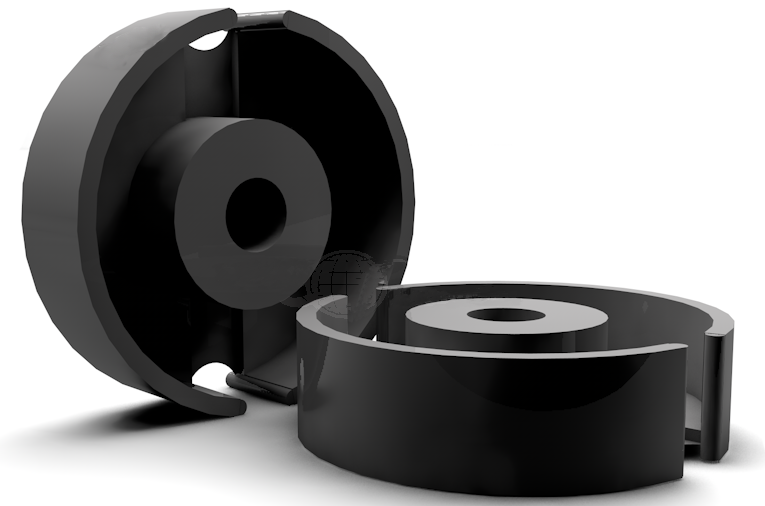
\includegraphics[width=0.35\linewidth]{pot_core.png}
            \captionof{figure}{Hrníčkové jádro}
            \label{ES:fig_001}
          \par}
          
          Kvůli redukci ztrát v jádře volíme dovolené maximální sycení \(B_m\) pouze 
          \SI{0.1}{\tesla} (dovolená hodnota pro daný materiál je cca \SI{0.35}{\tesla}, 
          závisí na teplotě).
    \item Potřebný počet závitů cívky dle:
          \begin{equation*}
            N = \frac{LI_{max}}{B_{max}S}
              = \frac{\num{.32d-6}\cdot\num{147}}{\num{.1}\cdot\num{265d-6}}
              = \num{1.78}
          \end{equation*}
          Pro snadnou realizaci voleno \(N = \num{1.5}\) závitu. Maximální indukce pak bude 
          asi \(\SI{0,12}{\tesla}\).
    \item Vzduchová mezera v jádře musí mít dle (\ref{ES:eq_009}) délku:
          \begin{align*}
            l_v &= \left(\frac{N^2}{L}-\frac{1}{\Lambda}\right)\mu_0           \\
                &= \left(\frac{\num{1.5}^2}{\num{.32d-6}}-
                   \frac{1}{\num{8980d-9}}\right)\num{4\pi d-7}\,\num{265e-6}  \\
                &= \SI{2.3}{\mm}
          \end{align*}
          Realizujeme ji zabroušením středního sloupku jádra.
          Průřez mědi svazku tvořícího vodič vinutí pak musí být:
          \begin{equation*}
            S_v = \frac{I_{ef}}{J} = \frac{\num{56}}{\num{2.3}} = \SI{24.6}{\square\mm}
          \end{equation*}
          Hloubka vniku při kmitočtu \(f = \SI{180}{\kHz}\) bude:
          \begin{equation*}
            \delta = \frac{\num{75}}{\sqrt{f}} 
                   = \frac{\num{75}}{\sqrt{\num{180d3}}} = \SI{.18}{\mm}
          \end{equation*}
          Průměr jednoho drátu svazku tedy smí být maximálně \(2\delta\) tj. \SI{.36}{\mm}. 
          Použijeme vodič \texttt{CuL} s průměrem \SI{.355}{\mm}. Průřez drátu je dán vzorcem 
          \(S_1 = \frac{1}{4}\pi d^2\). Z poměru \(\frac{S_v}{S_1}\) určíme počet vodičů  ve 
          svazku:
          \begin{equation*}
            n = \frac{4S_v}{\pi d^2} 
              = \frac{\num{4}\cdot\num{24.6}}{\pi\cdot\num{.355}^2}
          \end{equation*}
    \item Průměr takto vytvořeného svazku i s vnější izolací bude odhadem asi \SI{7.5}{\mm}.
          Rozměry okénka jádra jsou \(\num{20.3}\times\SI{8.95}{\mm}\). Při tloušťce 
          kostřičky cca \SI{1.5}{\mm} lze počítat s okénkem pro vinutí o rozměrech 
          \(\num{17.3}\times\SI{7.45}{\mm}\). Průřez tohoto okna je: 
          \begin{equation*}
            S_{okno} = \num{17.3}\cdot\SI{7.45}{\square\mm} = \SI{128}{\square\mm}
          \end{equation*}
          Vinutí má \num{1.5} závitu. To znamená, že v jedné polovině obvodu jsou v daném 
          okénku závity dva. Ve jmenované obvodu je tedy činitel plnění:
          \begin{equation*}
            k_{pl} = \frac{2S_v}{S_{okno}} 
                   = \frac{\num{2}\cdot\num{24.6}}{\num{128}} = \num{.38}
          \end{equation*}
          To je reálná hodnota i při našem způsobu vinutí (nikoliv volné vodiče do vrstev, 
          ale \num{1.5} závitu silným předem vyrobeným svazkem s vnější izolací). Vinutí se 
          dobře vtěsná, aniž by přitom zůstal velký prostor nevyužit. To je důkazem správné 
          počáteční volby velikosti jádra.
    \item Výpočet odporu vinutí:
          Měrný odpor mědi při předpokládané teplotě vinutí \SI{80}{\celsius}:
          \begin{align*}
            \varrho_{80} &= \varrho_{20}(1+\alpha\Delta t)  \\
                         &= \num{.0178}(1+ \num{4d-3}\cdot60)
                          = \SI{.22}{\ohm\square\mm\per\m}
          \end{align*}
          Délka jednoho závitu cívky: cca \SI{126}{\mm}\newline
          Délka celého vinutí i s přívody: \(l=\SI{250}{\mm}\) \newline
          Odpor vinutí při  \SI{80}{\celsius}:
          \begin{equation*}
            R = \varrho_{80}\frac{l}{S_v} 
              = \num{.022}\frac{\num{.25}}{\num{24.6}} = \SI{2.24d-4}{\ohm}
          \end{equation*}
          Ohmické ztráty na vinutí při \(I_{ef}\):
          \begin{equation*}
            P_{Cu} = R_{Cu}I_{ef}^2 = \num{2.24d-4}\cdot\num{56}^2 = \SI{.7}{\watt}
          \end{equation*}
          Hysterezní ztráty v jádře:\newline
          Katalogový údaj pro dané jádro: \(P_{h0} = \SI{3}{\watt}\) při \(f_0 = 
          \SI{15}{\kilo\Hz}\) a \(B_0 = \pm\SI{.2}{\tesla}\)
          \begin{align*}
            P_{h}   &= \frac{1}{4}P_{h0}\left(\frac{B}{B_0}\right)^2\frac{1}{T_{ekv}\cdot f} \\
                    &= \frac{1}{4}\cdot\num{3}\left(\frac{\num{.12}}{\num{.2}}\right)^2
                       \frac{1}{\num{12.7d-6}\cdot\num{15d3}} = \SI{1.4}{\watt}              \\
            \shortintertext{Celkové ztráty:}
            P_{tot} &= P_{Cu} + P_{h} = \num{.7} + \num{1.4} = \SI{2.1}{\watt}
          \end{align*}
  \end{enumerate}
\end{example}
  
      %-------------------------------------------
    
  \newpage
  \section{Vodiče}
    Nejčastěji se pro vinutí tlumivek a transformátorů používají lakované vodiče LC z měkké 
    elektrovodné mědi. Tepelná třída je určena druhem izolace, která je uvedena v normě. 
    Samopájitelné laky s polyuretanovou izolací jsou pro teplotní třídu B (\SI{130}{\celsius})
    
  \subsection{Efektivní hodnoty proudů typických prů\-bě\-hů}
    Pro správnou volbu průřezu drátu pro vinutí je nutné stanovit přípustné oteplení, které je 
    určeno efektivní hodnotou proudu. Pro nejčastější průběhy proudů jsem odvodil vztahy pro 
    výpočet efektivních hodnot.

    \begin{enumerate}
      % 1) =========================================================================================
      \item Výpočet efektivní hodnoty proudu s průběhem na obrázku \ref{es:fig_current_ef_solve_1}:
        {\footnotesize
          \begin{align}\label{es:eq_Ief1_solve}
            I_{ef}^2 &= \frac{1}{T}\int_0^{\delta T}i^2(t)dt=
                        \frac{1}{T}\int_0^{\delta T}
                                          {\left(\frac{I_{max}}{\delta T}t\right)^2}dt \nonumber \\ 
                     &= \frac{1}{T}\left(\frac{I_{max}}{\delta T}\right)^2
                        \int_0^{\delta T}{t^2}dt =
                        \frac{1}{T}\left(\frac{I_{max}}{\delta T}\right)^2
                                   \left[\frac{t^3}{3}\right]_0^{\delta T}             \nonumber \\ 
                     &= \frac{1}{T}\frac{I_{max}^2}{(\delta T)^2}
                        \frac{(\delta T)^3}{3}=I_{max}^2\frac{\delta}{3}
          \end{align}
        } %
        \begin{figure}[hp!]
          \centering
          \subfloat[$I_{ef}=I_{max}\sqrt{\frac{\delta}{3}}$]{\label{es:fig_current_ef_solve_1}
            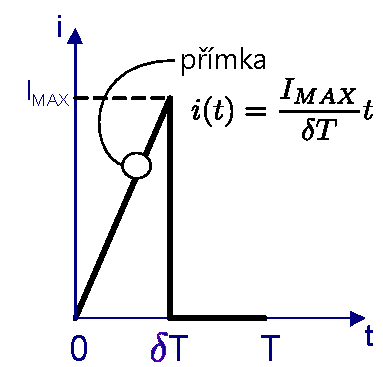
\includegraphics[width=0.3\linewidth]{current_ef_solve_1.pdf}}
          \subfloat[$I_{ef}=I_{max}\sqrt{\frac{1}{3}}$]{\label{es:fig_current_ef_solve_2}
            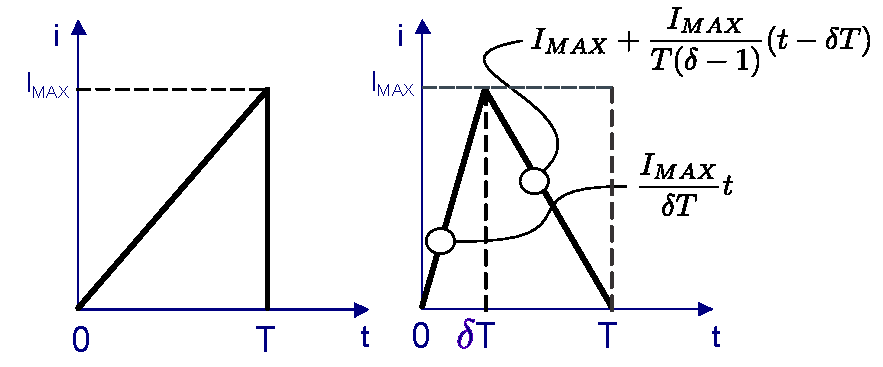
\includegraphics[width=0.6\linewidth]{current_ef_solve_2.pdf}}
          \caption{Typické průběhy proudů, jejichž efektivní hodnotu je nutné stanovit při 
                   dimenzování vinutých komponent.}
          \label{es:fig_Ief_solve1}
        \end{figure}
      % 2) =========================================================================================
      \item Výpočet efektivní hodnoty proudu s průběhem na obrázku \ref{es:fig_current_ef_solve_2}:
            Pravý průběh na obrázku \ref{es:fig_current_ef_solve_2} je speciálním případem levého
            průběhu jehož efektivní hodnotu snadno určíme jako $I_{max}\sqrt{\frac{1}{3}}$. Pro
            úplnost proveďme výpočet následujícím způsobem
        \begin{align}\label{es:eq_Ief2_solve}
          I_{ef}^2 &= I_{ef1}^2+I_{ef2}^2                                   \nonumber \\
                   &= I_{max}^2\frac{\delta}{3}+I_{max}^2\frac{1-\delta}{3}
                    = I_{max}^2\frac{1}{3}
        \end{align}
        výpočet dílčí efektivní hodnoty proudu $I_{ef2}$:
        {\footnotesize
          \begin{align*}
            I_{ef2}^2 &=  \frac{1}{T}\int_{\delta T}^{T}{\left(I_{max}+
                          \frac{I_{max}}{T(\delta - 1)}(t-\delta T)\right)^2}dt           \\ 
                      &   \left(\begin{array}{ccc}
                             \tau=t-\delta T  &  \Rightarrow  & \tau_h = T(1-\delta)  \\
                            d\tau=dt          &  \Rightarrow  & \tau_d = 0
                          \end{array}\right)                                              \\
                      &=  \frac{1}{T}\int_0^{T(1-\delta)}{\left(I_{max}+
                          \frac{I_{max}}{T(\delta-1)}\tau\right)^2}d\tau                  \\ 
                      &=  \frac{1}{T}\int_0^{T(1-\delta)}\left({I_{max}^2+
                          \frac{2I_{max}^2}{T(\delta-1)}\tau+
                          \left(\frac{I_{max}}{T(\delta-1)}
                          \right)^2}\tau^2\right)d\tau                                    \\  
                      &=  \frac{I_{max}^2}{T}\left[{\tau+\frac{2}{T(\delta-1)}
                          \frac{\tau^2}{2}+\left(\frac{1}{T(\delta-1)}\right)^2
                          \frac{\tau^3}{3}}\right]_0^{T(1-\delta)}                        \\ 
                      &=  \frac{I_{max}^2}{T}\left(T(1-\delta)-T(1-\delta)+
                          \frac{T}{3}(1-\delta)\right)                                    \\ 
                      &=  I_{max}^2\frac{1-\delta}{3}                                     \\ 
          \end{align*}
        } %
      % 3) =========================================================================================
      \item Výpočet efektivní hodnoty proudu s průběhem na obrázku \ref{es:fig_current_ef_solve_3}:
          \begin{figure}[hpt!]
            \centering
            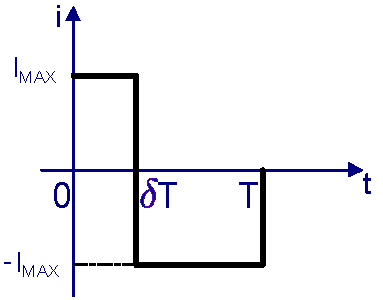
\includegraphics[width=0.5\linewidth]{current_ef_solve_3.pdf}
            \caption{\(I_{ef} = I_{max}\)}
            \label{es:fig_current_ef_solve_3}
          \end{figure}
        
      % 4) =========================================================================================
      \item Výpočet efektivní hodnoty proudu s průběhem na obrázku \ref{es:fig_current_ef_solve_4}:
        \begin{equation}\label{es:eq_Ief4_solve}
            I_{ef}=\sqrt{I_{ef1}^2+I_{ef2}^2}=\sqrt{2I_{max}\delta}
        \end{equation}
        {\footnotesize
          \begin{equation}\label{es:eq_Ief4}
              I_{ef1}^2=I_{ef2}^2
                      =\frac{1}{T}\int_0^{\delta T}{I_{max}^2}dt           
                      =\frac{1}{T}I_{max}^2[t]_0^{\delta T}=I_{max}^2\delta
          \end{equation}
        } %
        \begin{figure}[ht!]
          \centering
          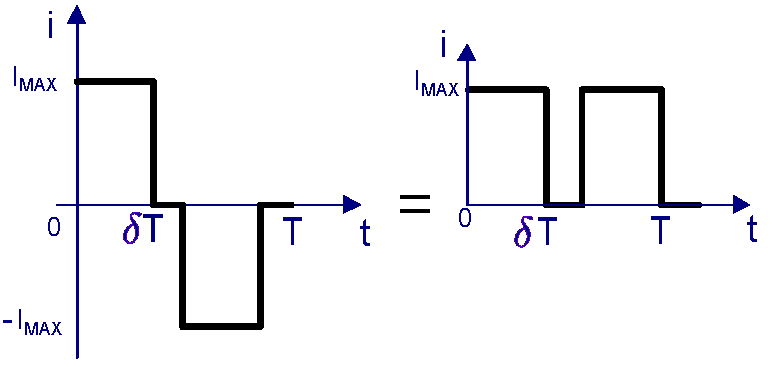
\includegraphics[width=0.7\linewidth]{current_ef_solve_4.pdf}
          \caption{$I_{ef}=I_{max}\sqrt{2\delta}$}\label{es:fig_current_ef_solve_4}
        \end{figure}

      % 5) =========================================================================================
      \item Výpočet efektivní hodnoty proudu s průběhem na obrázku \ref{es:fig_current_ef_solve_7}:
          \begin{equation}\label{es:eq_current_ef_solve_7}
            I_{ef}^2 = \frac{1}{T}\int_0^{\delta T}{I_{max}^2}dt 
                     = \frac{1}{T}I_{max}^2[t]_0^{\delta T}=I_{max}^2\delta
          \end{equation}

          \begin{figure}[ht!]
            \centering
            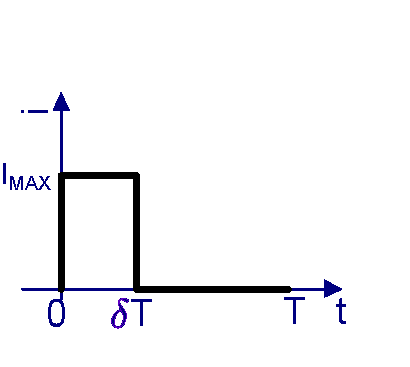
\includegraphics[width=0.6\linewidth]{current_ef_solve_7.pdf}
            \caption{ }
            \label{es:fig_current_ef_solve_7}
          \end{figure}
        
      % 6) =========================================================================================
      \item Výpočet efektivní hodnoty proudu s průběhem na obrázku \ref{es:fig_current_ef_solve_5}:
         {\footnotesize
          \begin{align*}
            I_{ef}^2 
              &=  \frac{1}{T}\int_0^{\delta T}\left(I_{max}-I_n + 
                  \frac{I_n}{\delta T}t\right)^2dt                                 \\                   
              &=  \frac{1}{T}\int_0^{\delta T}\left((I_{max}-I_n)^2t + 
                  \frac{2I_n(I_{max}-I_n)}{\delta T}t +
                 (\frac{I_n}{\delta T})^2t^2\right)dt                              \\ 
              &=  \frac{1}{T}\left((I_{max}-I_n)^2t +
                  \frac{I_n(I_{max}-I_n)}{\delta T}t^2 +
                 (\frac{I_n}{\delta T})^2\frac{t^3}{3}\right)_0^{\delta T}         \\ 
              &=  \frac{1}{T}\left((I_{max}-I_n)^2\delta T +
                  \frac{I_n(I_{max}-I_n)}{\delta T}\delta T^2 + 
                 (\frac{I_n}{\delta T})^2\frac{\delta T^3}{3}\right)               \\  
              &=  \delta\left((I_{max} - I_n)^2 + I_n\cdot(I_{max}-I_n) +
                  \frac{I_n}{3}^2\right)                                           \\  
              &=  \delta\left(I_{max}^2-2I_{max}I_n+I_{n}^2 + I_{max}I_n-I_n^2 +
                  \frac{I_n^2}{3} \right)                                          \\ 
              &=  \delta\left(I_{max}^2-I_{max}I_n+\frac{I_n^2}{3}\right)
          \end{align*}
          } %
        \begin{figure}[ht!]
          \centering
          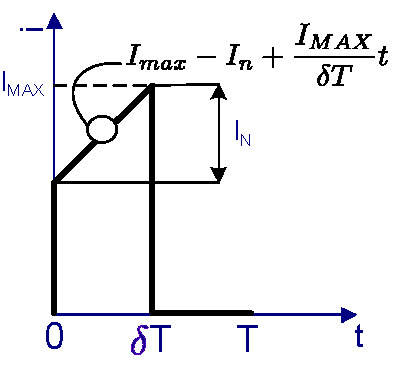
\includegraphics[width=0.5\linewidth]{current_ef_solve_5.pdf}
          \caption{\(I_{ef}=I_{max}\sqrt{\delta\left(I_{max}^2+\frac{I_n^2}{3}- 
                   I_nI_{max}\right)}\) }
          \label{es:fig_current_ef_solve_5}
        \end{figure}        
         
      % 7) =========================================================================================
      \item Výpočet efektivní hodnoty proudu s průběhem na obrázku \ref{es:fig_current_ef_solve_6}:
        {\footnotesize
          \begin{align*}
            I_{ef1}^2 &=  \delta\left(I_{max}^2-I_{max}I_n+\frac{I_n^2}{3}\right)         \\
            I_{ef2}^2 &=  \frac{1}{T}\int_{\delta T}^{T(1-\delta)}\left(I_{max}
                         +\frac{I_n}{T(\delta-1)}(t-\delta T)\right)^2dt                  \\
                      &=  \text{meze:}\left(
                            \begin{array}{cc}
                                \tau = t -\delta T & \tau_h = T(1-\delta)  \\
                               d\tau = dt          & \tau_d = 0
                            \end{array}
                          \right) \\ \nonumber
                      &=  \frac{1}{T}\int_0^{T(1-\delta)}\left(I_{max} +
                          \frac{I_n}{T(\delta-1)}\tau\right)^2d\tau                       \\
                      &=  \frac{1}{T}\int_0^{T(1-\delta)}\left(I_{max}^2 +
                          \frac{2I_{max}I_n}{T(\delta-1)}\tau +
                          \left(\frac{I_n}{T(\delta-1)}\right)^2\tau^2\right)d\tau        \\
                      &=  \frac{1}{T}\left[I_{max}^2\tau +
                          \frac{I_{max}I_n}{T(\delta-1)}\tau^2 +
                          \left(\frac{I_n}{T(\delta-1)}\right)^2
                          \frac{\tau^3}{3}\right]_0^{T(1-\delta)}                         \\
                      &=  (1-\delta)\left[I_{max}^2+I_{max}I_n - \frac{I_n^2}{3}\right]
         \end{align*}
        } %
         \begin{figure}[ht!]
           \centering
           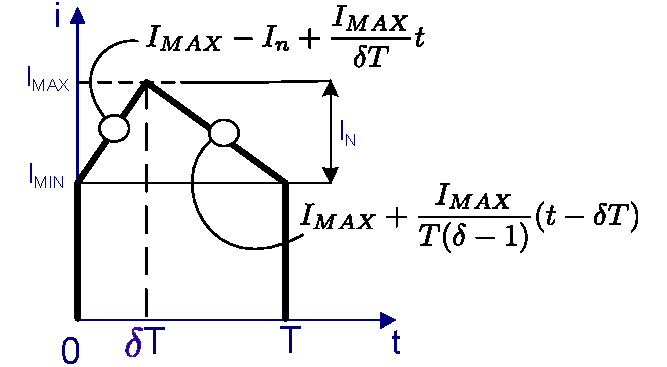
\includegraphics[width=0.3\textwidth]{current_ef_solve_6.pdf}
           \caption{\(I_{ef} = \sqrt{I_{ef1}^2+I_{ef2}^2} = \sqrt{I_{max}^2+I_{max}I_{n} - 
                    \frac{I_n^2}{3}}\) }
           \label{es:fig_current_ef_solve_6}
         \end{figure}

      % 8) =========================================================================================
      \item Výpočet efektivní hodnoty proudu s průběhem na obrázku \ref{es:fig_current_ef_solve_8}:
        {\footnotesize
          \begin{align*}
            I_{ef}^2 
              &=  \frac{1}{T}\int_0^{\delta T}{\left(I_{max}\sin(t)\right)^2}dt=
                  \frac{I_{max}^2}{T}\int_0^{\delta T}{\sin^2(t)}                          \\ 
              &=  \frac{I_{max}^2}{T}\left[\frac{t}{2}-
                  \underbrace{\frac{\sin(t)\cos(t)}{2}}_{\sin(\delta T)=0}\right]_0^{\delta T}
                  = I_{max}^2\frac{\delta}{2}                                              \\
          \end{align*}
         } %
        \begin{figure}[ht!]
          \centering
          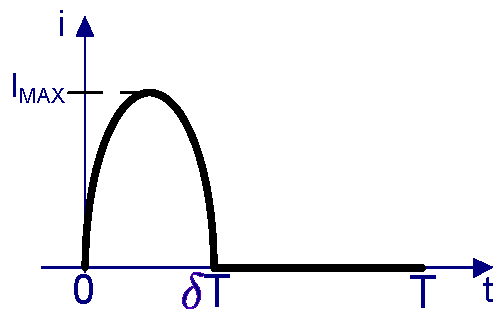
\includegraphics[width=0.3\textwidth]{current_ef_solve_8.pdf}
          \caption{\(I_{ef} = I_{max}\sqrt{\frac{\delta}{2}} \)}
          \label{es:fig_current_ef_solve_8}
        \end{figure}

    \end{enumerate}

} % tikzset
%---------------------------------------------------------------------------------------------------
\printbibliography[title={Seznam literatury}, heading=subbibliography]
\addcontentsline{toc}{section}{Seznam literatury}